% !TeX spellcheck = da_DK
\subsection{Software}
Efter det digitale signal er sendt igennem USB-isolatoren, indsendes de opsamlede data til en computer. Jævnfør afsnit \ref{subsec:software}, side \pageref{subsec:software} skal patienternes data behandles i form af grafisk visualisering af deres hældningsresultater, samt gemmes til senere brug og analyse. For at imødekomme disse krav, anvendes en computer med programmet Matlab. I Matlab designes en GUI (Graphical User Interface), hvor signalet fra accelerometeret visualiseres. Signalet optages i Matlab via NIDAQ'en. Grunden til der designes en GUI er for at optimere brugervenligheden. I GUI'en ses en graf, samt fire knapper og en toolbar, dette er illustretet på \figref{Fig:GUI_generisk}. 
\begin{figure}[H] 
	\centering 
	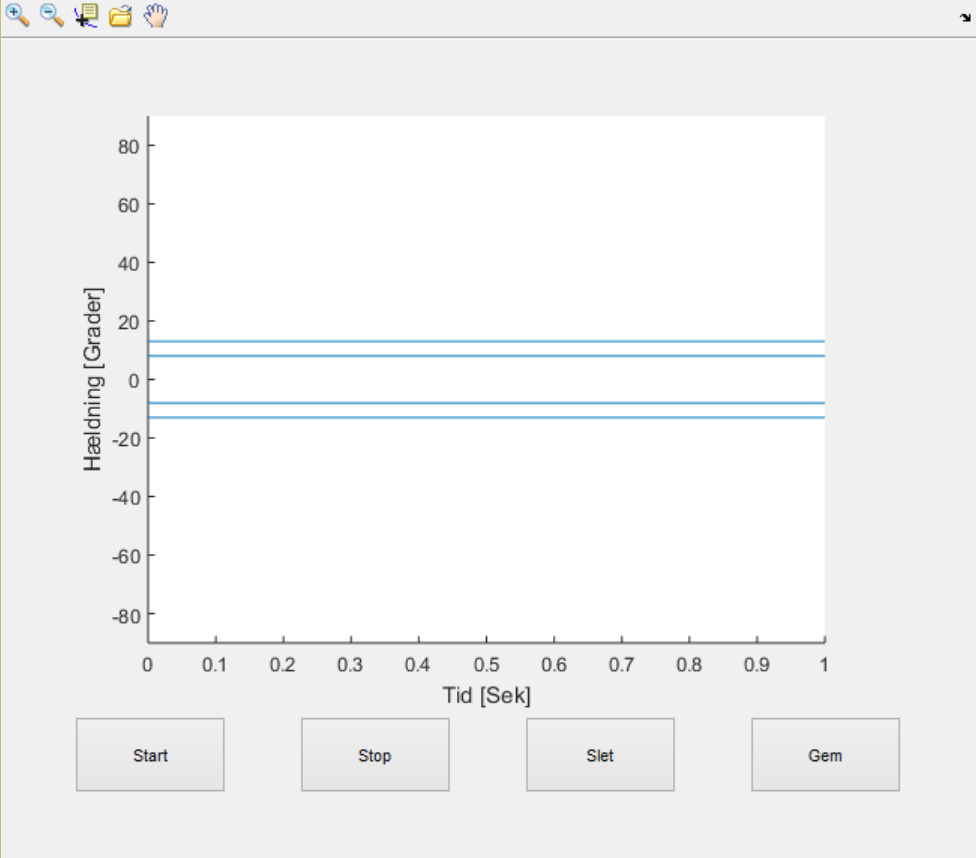
\includegraphics[scale=0.5]{figures/cProblemloesning/GUI_generisk.PNG}
	\caption{Af figuren fremgår GUI'ens standardvindue.}
	\label{Fig:GUI_generisk}
\end{figure} 
Y-aksen er defineret i grader, mens x-aksen er defineret i tid. Dette vil gøre at det bliver let at se i hvilken position patienten har befundet sig, samt i hvor langt tid.
De fire blå linjer på tværs af koordinatsystemet er de tærskelværdier vi har opstillet, som befindes sig i $\pm 8\circ$ og $\pm 13\circ$. Derved er det hurtigt for personalet at se hvor grænserne er for patienten.
Knappen start vil starte optagelsen af signalet. Knappen stop vil stoppe optagelsen af signalet. Knappen slet vil slette plottet af signalet. Knappen gem vil gemme figuren til senere analyse.
I toolbaren er der flere knapper, disse har til opgave at gøre det muligt at manipulere med grafen. Forstørrelsesglasset med plusset gør det muligt at zoome ind på grafen, men forstørrelsesglasset med minusset gør det muligt at zoome ud igen. Knappen med et papir og et plus gør det muligt at aflæse det præcise punkt på grafen som man vælger. Mappen der åbner gør det muligt at åbne en fil i GUI'en og hånden gør det muligt at panorere i grafen.
For at benytte GUI'en skal det fagkyndige personale åbne sciptet
Det fagkyndige personale skal åbne scriptet 'Patient_Oevelse' i Matlab for at kunne køre programmet, der skal behandle apopleksipatienternes data fra Scopelogger. Indsamlede data navngives efter den pågældende øvelse og dato og hentes ind i Matlab. Af \figref{Flow_manual} fremgår computerprogrammets manual som et flowdiagram.



\subsubsection{Test}
%Her skal det testes, hvorvidt systemet kan hvad vi beskriver det skal kunne.
%- Opsamling af noget data, hvor vi efterfølgende tester om programmet behandler dataen som det var tænkt.



%Vi kunne for at gøre programmet mere brugervenligt udarbejde en manual til systemet. Derudover kunne det være fordelagtigt at det fagkyndige personalet at have mulighed for at ændre akserne, og her tænkes specielt tidsaksen. Dette tænkes da systemet skal kunne optage selvtræning og da det ikke forventes at patienten tænder og slukker systemet efter hver enkelt øvelse. Dette vil både være svært at huske for patientgruppe (gamle og måske med kognitive komplikationer) og så ville de måske glemme at slå den til igen. Derfor tænkes det at de lader systemet optage signaler under hele selvtrænings sessionen. Det vil midlertidigt blive til utrolig meget data, hvor en stor del af dataen vil være pauser for patienten og derved ubrugelig data for det fagkyndige personale. Det ville derfor være smart at hvis de forholdsvis nemt kunne udvælge perioder i dataen, de gerne vil undersøge nærmere. 
%Derudover skal vi også have gjort patienten og det fagkyndige personale opmærksomme på hvilken øvelse der foretages!
%Det kunne måske være en ide, at vi i grafen kunne ligge tærskelværdierne ind som en form for linjer, så det blev nemmere at aflæse grafen
%Skal vi have en løbende visning af signalet i en graf eller er det bare til sidst! 

%Vores program skal altså kunne:
%  -Optage signalet
% - Behandle signalet således, alt efter sværhedsgrad 
%  - Plotte signalet
% - Gem data'en 
